The tunneling effect occurs when a particle faces a potential barrier. In the classical picture the particle is prohibited to move across the potential barrier if the particle's energy is lower than the barrier height. In quantum mechanics however, the particle is described as wave. When this now faces the potential barrier, a fraction of the wave package is transmitted through the barrier - an effect called tunneling.

\subsection{An historic overview}
The tunneling effect was first observed by Hund in 1926 in molecules, where he explained the sharing of an electron between atoms, each separated by a potential well.\cite{Mehra_tunneling_1982} A principle fundamental for an understanding of covalent chemical bonds. 

The first quantitative expression of the tunneling current between two vacuum separated metals was introduced by Bardeen in 1961.\cite{Bardeen_tunneling_1961} 

This lead to an early experiment build by Russell Young, John Ward and Fredric Scire in 1972.\cite{Young_topographiner_1972} Here tunneling with metal tip was shown already. The concept was further improved by Binning \& Rohrer in 1981 when they were the first to report experimental evidence for the tunneling through an vacuum gap.\cite{binning_tunneling_1982} They showcased the excelled resolution capabilities by resolving the ($7 \times 7$) reconstruction of the Si(111) surface \cite{binnig_1983} and received the noble prize in 1986 for "their design of the scanning tunneling microscope" (STM).\cite{_noble_price_1986} 

\subsection{Basic principles}
\index{STM!One dimensional tunneling}
In the following the tunneling process through a vacuum gap between metallic tip and sample will be summarized, addressed theoretically and used to describe the basic concept of STM.
\begin{figure}[]\centering
	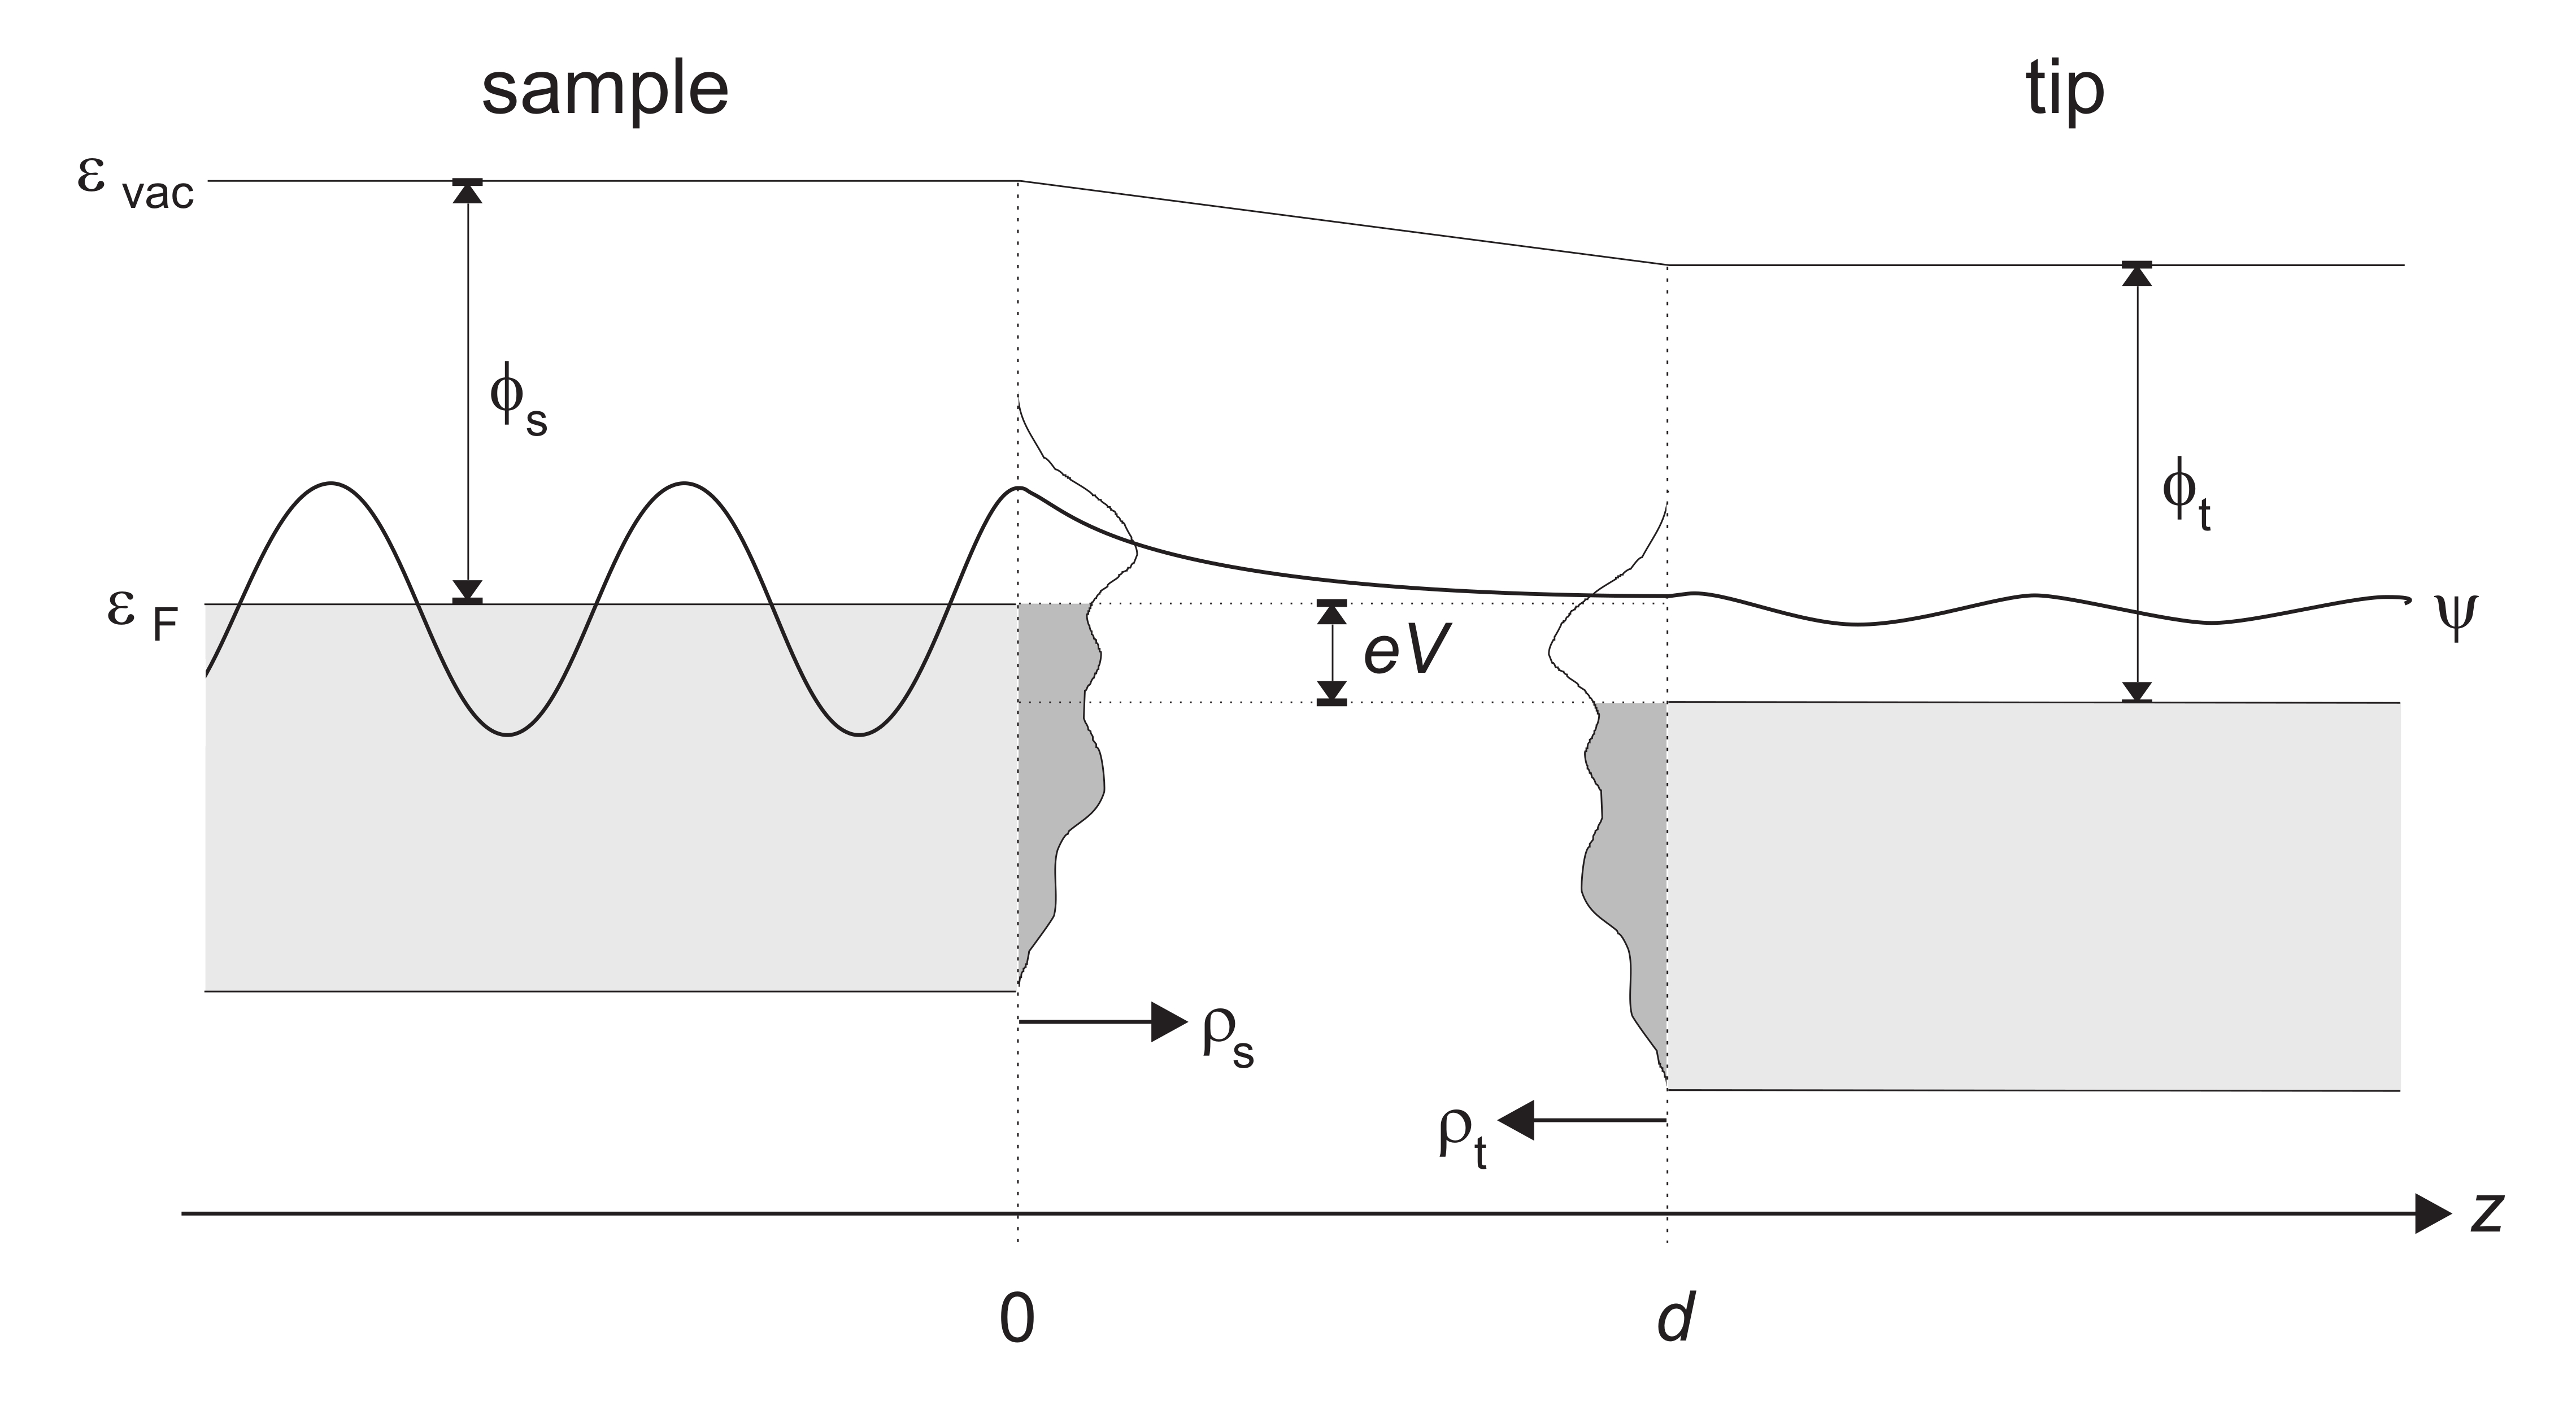
\includegraphics[width=0.7\textwidth]{./images/tunnel-barrier}
	\caption{Energy diagram to visualize the tunneling process between sample (left) and tip (right) separated by a distance d. Work functions of sample and tip ($\Phi_s$ and $\Phi_t$) separate the filled states (shaded regions) and the vacuum level ($\epsilon_{vac}$). Since sample ($\rho_s$) and tip DOS ($\rho_t$) may not be uniform, a fictional DOS is sketched in darker colors between both. The samples energy is lifted by $eV$ after a bias is applied and results in a net electron current from the sample into the tip. One tunneling process is indicated by a wave function $\Psi$. After overcoming the vacuum barrier its amplitude decreased and the corresponding electron occupies a free state (white background) in the tip material.  Adopted from \cite{diss-schunack}}
	\label{fig:STM-barrier}
\end{figure}

Consider a system where two metals (sample and tip) are separated by a vacuum gap. 

The amount of energy needed to remove an electron from the metals highest occupied energy level ($E_F$, Fermi energy) is called work function $\Phi$. It depends on the electrostatic potential $\phi_E$ that has to be overcome by an electron with charge $e$ at the surface.
$$ \Phi = -e \phi_E - E_F $$

\autoref{fig:STM-barrier} shows an energy diagram for tip and sample. The work function $\Phi_s$ (sample) and $\Phi_t$ (tip) separates the vacuum level $\epsilon_{vac}$ and Fermi energy $E_F$.

If sample and tip are in thermodynamic equilibrium, their Fermi energies are equal.
When both are brought in close contact, electrons from the sample tunnel into unoccupied states of the tip and vice versa with the same probability. Hereby electrons close to $E_F$ have the largest decay length 
%and attenuate less strong in vacuum 
and contribute strongest to the tunneling current. This current can be modeled and calculated in simple systems. 

%\paragraph{STM}
In the model of Tersoff-Hamann\index{STM!Tersoff-Hamann} the tip is atomically sharp and its electrons waveform is s-like.\footnote{Please's note that there are more models and corrections to them. An evolution from Bardeen's approach to the one done by Tersoff-Hamann can be found here \cite{lounis_theory_2014, wortmann_interpretation_2000} including Chen's expansion.} Further assuming low temperature and a constant band structure for the tip with apex radius R, it is possible to calculate the tunneling current $I$

\begin{figure}\centering
	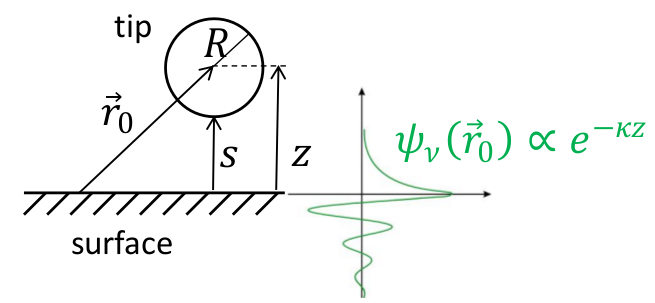
\includegraphics[width=0.7\textwidth]{./images/TH-tip-model}
	\caption{Left: Tersoff-Hamann geometry model for a tip with radius R  positioned at a distance s above the sample at position $\vec{r_0}$. Right: Exponential decay of electronic states at the sample surface into the vacuum. Image adopted from \cite{STM_theory_versuch_temirov}.}
	\label{fig:STM-TH_model}
\end{figure}

$$I \propto \frac{2 \pi e^2}{\hbar} \cdot U \cdot \rho_t(E_F) \cdot e^{2\kappa R} \rho_s(E_F,\vec{ r_0})$$

where $\rho_s(E_F,\vec r_0)$ is the LDOS of the sample at $E_F$, evaluated at position $\vec{r_0}$.

With this theory constant current STM images the surface density of states for  a given voltage $U$. 
$$\rho_s(E_F,\vec r_0)= \rho_s(E) \cdot exp(-2\kappa (\underbrace{s+R}_{Z}))$$
The exponential decay ($\propto e^{-\kappa Z}$) of an electron wave function into vacuum is characterized by $\kappa=\frac{\sqrt{2m\Phi}}{\hbar}$. It limits the current, which is proportional to the squared amplitude of it. 
$$I\propto e^{-2\kappa Z}$$
Like in one dimension the current depends on the barrier height $\Phi$ through $\kappa$. Increasing the distance exponentially decreases the tunneling current.
%\footnote{\url{http://pmrb.free.fr/work/diplom/html/mainse2.html} }% 
This exponential relation is the reason for the excellent topography resolution capabilities of STM. While its a good first approximation of the system, in many cases more than just the electrons near Fermi contribute. Also a uniform $\rho_t(E)$ may not be accurate in all cases.

Using \index{STM!WKB} Wentzel-Kramers-Brillouin (WKB) theory\cite{wentzel_verallgemeinerung_1926, kramers_wellenmechanik_1926, brillouin_mecanique_1926} the tunneling current is given by
\begin{equation}
I=\int_0^{eU}\rho_s(r,E)\rho_t(r,eU+E)T(E,eU,r)dE
\label{WKB}
\end{equation}
where %$\rho_s(\rho_t)$ is the density of states of the sample (tip) and %
T is the tunneling transmission probability
\begin{equation}
T(E,eV)=exp\left(-\frac{s\sqrt{2m}}{\hbar}\sqrt{\frac{\Phi_s+\Phi_t}{2}+\frac{eU}{2}-E}\right)=exp\left(-2\kappa_{eff}(E,U)s\right)
\label{Transmission-function} 
\end{equation}
describing the probability of an electron tunneling event between tip and sample.

The samples potential can be changed by applying a voltage $V=U_b$ (bias) to it. This lifts its Fermi energy with respect to the tips and leads to a net electron current from the sample into the tip. Inverting the voltage results in electrons tunneling from the tip into the sample. If $eV<0$ the tunneling current is largest for $E=0$ (electrons on the Fermi-level of the sample), if $eV>0$ the tunneling current is largest for $E=eV$ (electrons of Fermi level in tip).

Due to the fact that the tunneling current is proportional the density of states in the tip and the sample one can deduce its band structure within a range of several volts in the vicinity of the Fermi energy. Investigation of this behavior led to the establishment of a new measurement technique, called scanning tunneling spectroscopy (STS).

\subsection{\textbf{S}canning \textbf{T}unneling \textbf{S}pectroscopy}
\label{section:STS}
Changes of the tunneling current with the bias voltage were observed by Tromp et al. in 1986 \cite{tromp_atomic_1986}. They discovered a change in contrast when scanning a SI(111) surface with either positive or negative bias. The change in contrast is most apparent in semiconductors and semi metals\cite{bonnell_scanning_1993}, but adsorbates and charged areas of the sample change the DOS locally and therefore the contrast in STM. While simple results may be already obtained by comparing two images recorded at different biases, more detailed information can be achieved.

\index{STS!Bias below work function}
If tunneling conditions are such that $eV\leq\Phi$, observed features in $dI/dV$ are associated with the surface DOS. Critical points in the surface projected DOS give rise to features in dI/dV. Interpretation of these features with the WKB theory (i.e. differentiating equation \eqref{WKB}) gives
\begin{equation}
dI/dV=\rho_s(r,eV)\rho_t(r,0)T(E,eV,r)+\int_0^{eV}\rho_s(eV)\rho_t(r,E-eV)\frac{dT(E,eV,r)}{dV}dE
\label{eq:dI/dV}
\end{equation}
The first term $\rho_s(r,eV)\rho_t(r,0)T(E,eV,r)$ contains the DOS of tip/sample and the transmission function. It describes the dependence on the DOS in the sample for energies $eV$ - our desired spectrum.  While T is usually unknown, a closer look to \eqref{Transmission-function} indicates a smooth, monotonically increasing function in V. This mannered dependence on V gives a smooth background described by the second term $\int_0^{eV}\rho_s(eV)\rho_t(r,E-eV)\frac{dT(E,eV,r)}{dV}dE$.
 As for STM topography images, bias voltage can be chosen to either probe occupied ($U_b < \SI{0}{\volt}$) or unoccupied states ($U_b > \SI{0}{\volt}$).  At low temperatures the vanishing lateral movement of adsorbates makes them also accessible to tunneling spectroscopy with sub molecular lateral resolution. 
 %It is possible to deduce the electronic configuration with atomic spatial resolution.

\subsection{Machine description and experimental details}
The success of STM and STS is promoted by good mechanical engineering. Since distances down to the atomic length scales are investigated, the experiment needs a careful set up. This is true especially for damping of external vibration that would otherwise conflict with the measurement. Sufficiently low partial pressures are needed to achieve small contaminant adsorption rates and the long investigation times associated with them. To conduct experiments in the most controlled environment possible, sample preparation and investigation is done in ultrahigh vacuum (UHV) chambers.

Since all used UHV chambers have many common parts, a typical setup is described with the low temperature (LT) STM setup, where most experiments were carried out.

The central part of the LT-STM setup is the commercial \textbf{Beetle-type STM scanner} \cite{zoephel_aufbau_2000} as shown in \autoref{fig:stm-heliocoidal-ramp}. Here a helicoidal ramp carries the central scan piezo with attached STM tip. Three outer piezo tubes are used in slip-stick motion to circularly move on the ramp. Because the ramp is cut with an inclination of \SI{2}{\degree} the circular motion of the piezos results in the STM tip moving up and down. This is used to control the height above the sample during tip approach and macroscopic lateral movement.

%A separate piezo is used to control the lateral position of the tip during scanning. With it the image width, scan speed and tip-sample distance can be controlled on a continuous, sub-atomic length scale (\autoref{fig:STM-tip}).

Not only the macroscopic movement of the STM stage is controlled with a set of piezos, but the position of the tip (x, y, z) during scanning, too (see \autoref{fig:STM-tip}). In this work a segmented tubular piezo is used to control the tips position. The piezos elongation can be controlled with the voltage applied to them, which is used to choose not only the tip-sample distance. Lateral movement is controlled by addressing its four segments. Each is used to control movement along $\pm \textnormal{x}$ and $\pm \textnormal{y}$ direction. %and controlled by the feedback loop. %
For recording an topographic image the area is raster scanned in consecutive lines, applying a sawtooth voltage to the fast scan direction. The next lines are chosen by stepwise increasing the voltage along the slow scan direction. Other parameters like image size and scan speed are controlled with the piezos as well.

The measured current is translated into a voltage (I/U converter) and processed in a 20 Bit analog $\rightarrow$ digital (A/D) converter. The current intensity is feed into the Digital signal processor (\textbf{DSP}) board. Here the STM Software's current set point is compared with the measured value. The tips position is controlled with a feedback loop. If the tips position needs to be corrected, a voltage is applied to the corresponding piezo element. 
%The DSP is used to attenuate high frequency components. \textcolor{red}{\textbf{ More detail?}}

Differentiation of the current signal is done with an \textbf{Lock-In Amplifier}. Here the spectrum is not recorded directly by sweeping the bias and numerically differentiating the measured current. A sinusoidal modulation on top of the bias voltage %with a frequency higher than the low pass frequency of the DSP 
is used. The modulated bias leads to a tunneling current modulation with the same frequency. The differentiation is performed by reading the AC current signal with the same frequency as the modulation which directly gives the dI/dV signal and therefore the DOS of the sample at $U_b$. Because the Lock-In Amplifier then only takes signals with the same frequency than the excitation frequency into account, the results are much less suspect to noise. Compared to numerical differentiation, a Lock-In needs less computing effort, too. It is important to note that the DSP does not recognize the bias/current modulation as topographic feature and regulates as without modulation. If the modulation frequency is too low, the feedback tries to compensate the modulation by changing the distance to the sample. If the modulation frequency is too high, the capacitance between tip and sample leads to an $90\deg$ phase shifted current which increases with modulation frequency. One usually chooses the modulation frequency slightly above the cutoff frequency for the feedback loop.

\begin{wrapfigure}{O}{5cm} \centering
	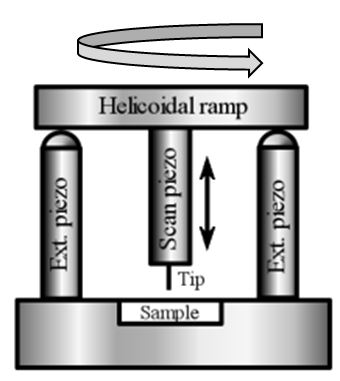
\includegraphics[width=4cm]{./images/STM-sketch-2}
	\caption{STM sample stage to control the tip position. The coarse movement is controlled by exterior piezos. Each moves on a heliocoidal ramp with slip-stick motion. The precise positioning during scan is done with a central piezo to which the tip is attached. Modified from \cite{heliocoidal_ramp_2018}.}
	\label{fig:stm-heliocoidal-ramp}
\end{wrapfigure}

The UHV setup for the LT-STM is shown in \autoref{fig:chamber-sketch}. With a base pressure of $\approx \SI{5e-10}{\milli \bar}$ these stainless steel chambers are almost free of contaminants. Since the rate at which residual gas contaminates the sample is proportional to the residual partial pressure, the time needed to cover the surface is proportional to it. When the base pressure is lowered by a factor of \SI{1e-13} (\SI{1}{\bar} $\rightarrow$ \SI{1e-10}{\milli \bar}), the time needed to cover the sample is increased by a factor \SI{e13}{}.

To maintain UHV conditions, a set of pumps is used. For the preparation chamber, where high partial pressures occur during sample cleaning and preparation, a combination of roughening and turbo molecular pumps is used. First a roughening pump lowers the atmospheric pressure to \SI{1}{\milli \bar}. With this pressure on the outlet side a turbo molecular pump is used to decrease the pressure even further to the  \SI{1e-8}{\milli \bar} range. The remaining pressure is caused by adsorbate covered chamber walls where continuous ad-/desorption takes place and maintains a pressure equilibrium. After heating the entire chamber to temperatures above \SI{120}{\celsius} while constantly pumping, most of the water is desorped from the walls and pumped. After cooling down to room temperatures, the pressure settles in the \SI{e-10}{\milli \bar} regime. 

As the pumping efficiency of turbo molecular pumps decreases for low pressures, each chamber is equipped with an ion getter pump. Here a high voltage \SIrange{1}{7}{\kilo \volt} is applied between two getter materials. Residual gas particles ionize in the strong electric field and are accelerated towards the plates. Here they impinge with high velocity and are buried deep in the plate material that they can't leave. The reduced number of residual gas particles results in a lower pressure.

To further reduce the number of potential contaminations, parts of the chamber can be cooled down with liquid nitrogen. Because of the great temperature gradient, gaseous residuals condense on the much cooler surface of the cooling trap and remain adsorbed while the temperature is kept low. Without refilling with liquid nitrogen the temperature slowly increases over time, so that the cooling trap looses pumping efficiency over time (usually after \SIrange{1}{2}{\hour}) and starts to release trapped contaminants.

A titanium sublimation pump is installed to evaporate titanium on demand. This covers the chamber walls and, due to its reactivity, binds residual gas molecules. After some time the reactivity diminishes and a new layer has to be evaporated. With short operation intervals once a day the base pressure of the UHV system can be improved permanently.

While LT-STMs may be operated with solely helium as coolant, it is more resource saving to only cool the direct proximity of the sample and the STM with He (boiling point: \SI{4.2}{\K}) and to suppress the heat flow out of the He cryostat with a second, surrounding nitrogen cryostat (boiling point: \SI{77}{\K}) as shown in \autoref{fig:STM-cryo}). This diminishes consumption of globally limited He. To maintain a temperature of \SIrange{5}{7}{\K}, one to two liters of liquid helium are evaporated a day, plus an additional amount of three to four liters liquid nitrogen. Evaporated helium is reclaimed in a closed circuit with a system of purifying and storage/cooling steps so that only a small amount of helium escapes the circuit and is lost.

Sample temperatures down to \SIrange{5}{7}{\K} allow for observations not possible at elevated temperature. Cooling not only reduces thermal drift in the piezo elements that are used to control the tip's position on the sample. Thermal energy at low temperature is not high enough for atoms or molecules to move on most substrates. Species mobile at room temperature (and therefor not representable at room temperature in the sub-ML regime) become immobile and accessible for ST microscopy and spectroscopy. ST spectra resolution is better at low temperatures.

\begin{figure}[ht]\centering
	\subfigure[LT-STM setup. Different functional groups are highlighted by colors. A low base pressure is achieved with a combined pumping system comprised of ion pumps and turbo molecular pumps (cyan). Sample holders are operated with a rotatable, variable temperature manipulator (green). Sample preparation is done in the preparation chamber (blue). After transfer to the LT-STM chamber (yellow) a gate valve is used to seal the LT-STM from remaining residual gas that may be present in the preparation chamber. The liquid helium/nitrogen bath cryostat (red) is used to maintain low temperatures (see \subref{fig:STM-cryo}). Vibration isolation of the frame is achieved with legs floating on pressurized cylinders (orange).]{
		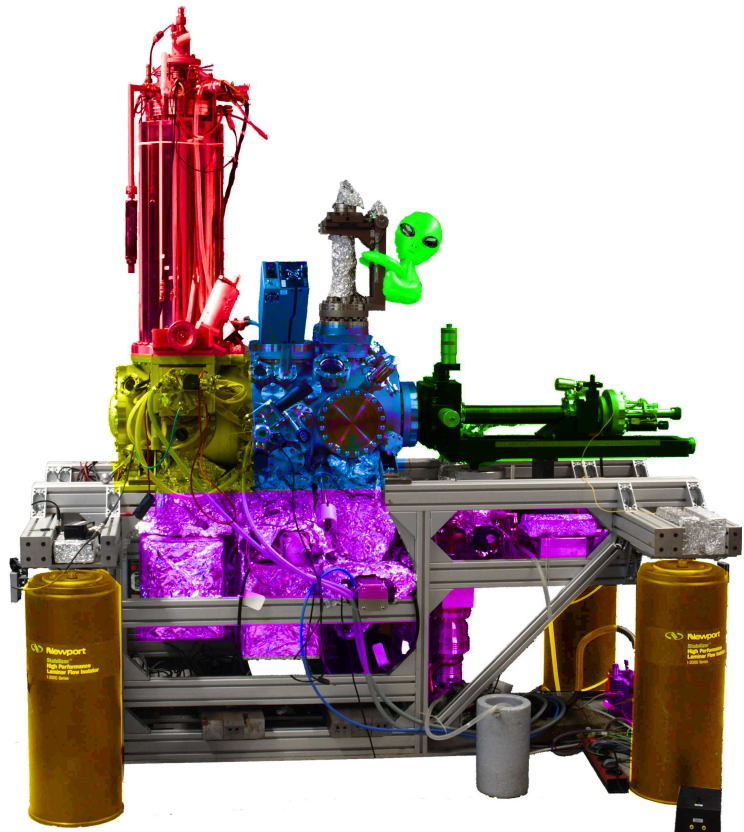
\includegraphics[width=0.45\textwidth]{./images/chamber-sketch.jpg}
		\label{fig:chamber-sketch}
	} \quad
	\subfigure[Scheme of a liquid bath cryostat. While in the inner stage a temperature of \SIrange{5}{7}{\K} is achieved with a liquid helium reservoir, an outer liquid nitrogen cryostat is used to isolate the inner cryostat from the surrounding room temperature and to reduce the amount of liquid helium used to maintain cryogenic temperatures.]{
		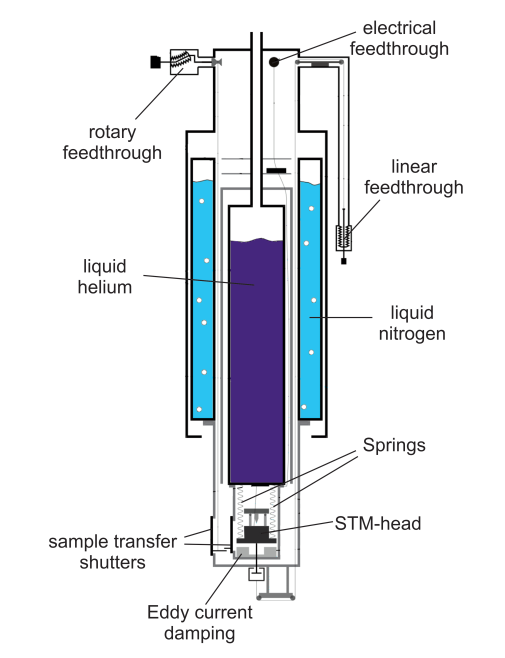
\includegraphics[width=0.45\textwidth]{./images/sketch-cryo.jpg}
		\label{fig:STM-cryo}
	}
	\caption{Typical setup for low temperature measurements. A vibration isolated UHV chamber is used to prepare samples and investigate them in a separable chamber with either STM or AFM. A liquid bath cryostat is used to maintain low temperatures. Images adopted from \cite{diss-knud}}
	\label{fig:STM}
\end{figure}

\begin{figure}\centering
	
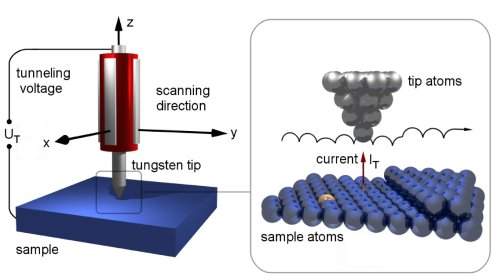
\includegraphics[width=0.6\textwidth]{./images/stm-rutgers-modified.jpg}
	\caption{Operating principles of a STM. A macroscopic sketch shows the central piezo that controls the tip position on the sample. The piezo is divided in four parts to control movement in the x-y plane and tip-sample distance. A microscopic sketch shows the tips movement in constant current mode while moving across a atomic step edge. Here the tip is retracted to maintain a constant current, which in turn leads to a larger apparent height in STM. Note the single incorporated alien atom. Although its height is the same as its neighbors, STM records the change in DOS. Less electrons tunnel and the apparent height on the terrace is reduced above the alien atom. Adopted from \cite{STM-rutgers}}
\label{fig:STM-tip}
\end{figure}

Two damping stages are used, one for the chamber and a sequential one for the STM.

First the whole UHV system is build within a frame that is placed on air pressurized cylinders. These can be lifted on demand, so that the chamber floats on four dampers and external vibrations/shocks are damped. Three legs are adjustable in height to level the whole setup properly.

A second stage decouples the sensitive STM scanner from the rest of the setup. First the complete STM stage hangs on springs to further limit the direct influence of vibrations. Second the remaining oscillation amplitude is damped by a eddy current damping. It is made of three magnets in close proximity to a surrounding conductor so that eddy currents are induced for each movement. The eddy current is typically larger at cryogenic temperatures, that results in a damping that works best at low temperatures. The kinetic energy of the oscillating system is transferred by the eddy currents into heat within the surrounding support. The heat is then mitigated by the external cooling of the cryostat.

\paragraph{Experimental details}

\textbf{Topography images} are created by raster scanning the surface pixel by pixel. 
We use the constant current (cc-STM) operating mode where the tips height is controlled to achieve a constant tunneling current as shown in \autoref{fig:STM-tip}. The regulating voltage on the height control piezo is recorded and plotted in a color-scale for each pixel. The brighter the color, the more the piezo had to retract the tip to maintain the constant tunneling current setpoint. Regions with the same DOS thus appear in the same contrast.

%	A modified tip allows for real space imaging of molecular orbitals.

Differential conductance measurements are performed in two ways - on single points (spectrum) and on areas (map). The feedback loop that controls the tip vertical position is not in use, so that the tip maintains a constant height that is set before measurement. \textbf{Single point spectra} are used to measure electronic properties like molecular orbital energies and electronic band gaps. Spectroscopic information is obtained by sweeping the bias voltage while recording the tunneling current (I(V,z)-spectroscopy) at constant tip-sample distance. Differentiation results in a term proportional to the DOS (see \autoref{eq:dI/dV}).
%or the tip-sample distance (V(z)-spectroscopy) with a fixed tunneling current.

\textbf{Spectral maps} at a fixed bias show real space distribution of electronic states at the DOS that corresponds to the chosen bias. The signal intensity represents the differential conductance $\propto$ DOS. Differentiation is done with a Lock-In.

For both types it is important to eliminate lateral and vertical drift, to ensure a fixed tip position above the point of interest during the measurement. This is even more important for spectral maps, since they take a long time to record.

\textbf{Lateral manipulation} of atoms and molecules is possible with the STM tip. With a matching current/voltage set point, the tips vertical position can be chosen such that the tip interacts with the adsorbate. Lateral displacement of single molecules within molecular assemblies is only possible if molecule-molecule interactions are weak, e.g. no covalent bonds are formed between molecules. If molecule-molecule interactions dominate, clusters of molecules are moved.

Experiments based on STM were done at different experimental chambers: 
(1) The described LT-STM chamber \cite{urgel_tendero_two-dimensional_2015, schwarz_assembly_2018, wiengarten_scanning_2015} and (2) a RT-STM with XPS capabilities described elsewhere.\cite{schwarz_assembly_2018}. 

The tip termination was changed in different ways. 
1. \textbf{Voltage pulse:} 
A voltage pulse ($U_b \leq \SI{10}{\volt}$) is given for a short time ($t \leq \SI{1}{\second}$) when the tip is in tunneling contact. The intense current pulse reorders the tip termination often leaving some tip adsorbates on the sample surface. While small pulses often only slightly change the tip geometry, larger pulses may lead to heavy rearrangements in tip and sample.
2. \textbf{Vertical over-approach:}
The tip is pushed into the sample surface in order to remove tip adsobates and aggregate sample surface atoms at the tip. While this works best for metallic samples, it should be avoided to accidentally cover the tip with insulating adsorbate layers as present for \textit{h}-BN preparations.
3. \textbf{Field emission:}
An external power supply is used to apply a voltage ($U_b$=
\SIrange{100}{500}{\volt}) between tip and sample. A serial resistor limits the current through the connected internal wires. Tip and sample are brought in close proximity to enable the tunneling process. Because of high electrical field strengths at the tip apex strong forces occur. Depending on the polarity the tip can either expel tip atoms or aggregate sample surface atoms. With a careful distance increase a new tip apex can be build up.
The above mentioned ways are done with the tip remaining inside the STM.
4. \textbf{Tip sputtering:}
To reorder the tip structure and to remove adsorbates accelerated Ar$^+$ ions are used. Because of higher partial pressures needed for sputtering the sample is transferred from the LT-STM into the preparation chamber. Here the tpi is bombarded with $Ar^+$ ions (\textcolor{red}{PARAMETERS}), annealed (\textcolor{red}{PARAMETERS}) and transferred back into the STM.

\subsection{Limitations}\index{STM:resolution}

The accuracy of a STM is very high with spatial resolution down to the atomic scale.

\textbf{Lateral resolution} with the STM depends on the tip shape and termination. A tip with single atom termination records sharp topography images. When there is more than one atom in the tip apex participating in the tunneling process, lateral resolution decreases and an image for each tip termination is created. This is often recognized by blurry step edges and artifacts that repeat several times within a single image.

\textbf{Spectral resolution} is influenced most by the tip DOS. Before each measurement a reference spectrum is recorded on the metal surface to ensure the the DOS of the tip is metallic and does not show unexpected additional states that are typically induced by a modified tip.

Due to the fact that the tips motion is controlled with different piezos, one has to take different elongations in different directions into account. For example, if the STM scans the fast scanning direction just a bit further than the slow scan direction, the resulting image (although pixel wise square) is no longer physically square anymore. 
%Imagine a square (1:1 side ratio, diagonal angle 45\textdegree) where one side is elongated by 5\%. The resulting square (1:1.05 side ratio, diagonal angle 43.6\textdegree) looks square because it has the equal number of pixels in both directions, but it is physically rectangular. The expression used to calculate the uncertainty with known calibration parameters is
%$$\Delta \Theta = 45 - \frac{180}{\pi}\cdot\arctan(\frac{1}{1+x})$$ where x is the percentage of one side being longer. This results in an uncertainty of 0.3\textdegree(1\%), 1.4\textdegree(5\%, see example above), 2.7\textdegree(10\%). 
For moderate shear below \SI{5}{\percent} however, conformity is almost conserved and the angular uncertainty below \SI{1.5}{\degree}.

Because STM is sensible to electronic changes, it may change the footprint of an adsorbed compound \cite{sautet_interpretation_1992}. Laterally approaching an adsorbate results in an additional tunneling current, because now electrons do not only tunnel directly into the substrate but through the adsorbate as well. Interferences between both tunneling processes depend on the adsorbate's orbital-symmetry and tip-shape. Local density of states calculations \cite{tersoff_theory_1985, lang_theory_1986, eigler_imaging_1991} are not adapted to grasp this effect since the tip is considered far away from the surface. Moreover, the tip radius or the tip-substrate distance is often optimized to fit the lateral size of the adsorbate print with the experimental image \cite{tersoff_theory_1985, eigler_imaging_1991}. 


Mechanical and thermal vibrations limit the resolution of STM and STS, too. Therefor the damping stages that decouple the STM from the surrounding are important but may not always filter all mechanical vibrations. 

Signal wires (coax) are well shielded against electromagnetic radiation. Since the signal is transmitted with cables an external radio signal may otherwise couple into the wire and tamper with the signal.

Although STM works at room temperature, additional cooling may be applied to reduce the thermal vibrations.

STM is not capable to discern different elements. As complimentary method, X-Ray photoelectron spectroscopy is used for convenient chemical identification of adsorbates.